\documentclass[a4paper, 11pt]{article} % Font size (can be 10pt, 11pt or 12pt) and paper size (remove a4paper for US letter paper)

\usepackage[protrusion=true,expansion=true]{microtype} % Better typography
\usepackage{graphicx} % Required for including pictures
\usepackage{hyperref}
\usepackage{float}

\usepackage[british]{babel}

\usepackage{mathpazo} % Use the Palatino font
\usepackage[T1]{fontenc} % Required for accented characters
\linespread{1.05} % Change line spacing here, Palatino benefits from a slight increase by default

\makeatletter
\renewcommand\@biblabel[1]{\textbf{#1.}} % Change the square brackets for each bibliography item from '[1]' to '1.'
\renewcommand{\@listI}{\itemsep=0pt} % Reduce the space between items in the itemize and enumerate environments and the bibliography

\renewcommand{\maketitle}{ % Customize the title - do not edit title and author name here, see the TITLE block below
\begin{flushright} % Right align
{\LARGE\@title} % Increase the font size of the title

\vspace{50pt} % Some vertical space between the title and author name

{\large\@author} % Author name
\\\@date % Date

\vspace{40pt} % Some vertical space between the author block and abstract
\end{flushright}
}

%----------------------------------------------------------------------------------------
%	TITLE
%----------------------------------------------------------------------------------------

\hyphenation{Phylo-Geo-Tool}

\title{\textbf{Phylogeotool}\\ % Title
Installation Manual} % Subtitle

\author{\textsc{Ewout Vanden Eynden, Pieter Libin, Kristof Theys, Guy Baele} % Author
\\{\textit{Rega Institute for Medical Research, KU Leuven}}} % Institution

\date{April 2017} % Date

%----------------------------------------------------------------------------------------

\begin{document}
\maketitle % Print the title section

\vspace{30pt} % Some vertical space between the abstract and first section

%------------------------------------------------
\tableofcontents
\newpage

%TODO (PL): spell check
%TODO (PL) mention which platforms are supported: windows, linux, macos
%-> Ewout is this correct.

\section{Installation}
\subsection{Prerequisites}
\subsection*{Java}
Install the Java Development Kit (JDK) with version $\geq 1.7$.\\

\noindent For example, on Ubuntu Linux, Oracle Java 8 can be installed as follows:
\begin{verbatim} 
sudo add-apt-repository ppa:webupd8team/java
sudo apt-get update
sudo apt-get install oracle-java8-installer
\end{verbatim}

\subsection*{Tomcat}
Install Tomcat version $\geq 7$.\\

\noindent For example, on Ubuntu Linux, Tomcat 7 can be installed as follows:
\begin{verbatim}
sudo apt-get update
sudo apt-get install tomcat7
\end{verbatim}

%TODO (PL): add R?

\subsection*{PPlacer and its dependencies}
 Install the python package manager \textbf{pip}. \\

\noindent For example, on Ubuntu Linux, \textbf{pip} can be installed as follows:
\begin{verbatim}
sudo apt-get install python-pip
\end{verbatim}

\noindent Install \textbf{taxtastic} as explained at \url{http://fhcrc.github.io/taxtastic/installation.html}.\\

\noindent Install \textbf{Mafft}  (TODO (Ewout): which version?) to align sequences to be classified by PPlacer. 
For example, on Ubuntu Linux, Mafft can be installed as follows:
\begin{verbatim}
sudo apt-get install mafft
\end{verbatim}

\noindent Install PPlacer (TODO (Ewout): which version) (website: \url{http://github.com/matsen/pplacer/releases}).

\subsubsection*{Phylogenetic tree}
A rooted phylogenetic tree in either Nexus or Newick format. It is important that the tree is \textbf{binary}.

\subsubsection*{CSV file}
A comma-separated value (CSV) file, containing an ID column that contains identifiers that correspond to the taxa names of the provided phylogenetic tree.
Remaining columns may contain additional information/annotation for the taxa in the phylogenetic tree. Examples of such annotations are: geographic location, virus genotype/subtype and patient attributes (age, ethnicity, \ldots). \\
Information on the geography of taxa can be visualized in a map (Google Charts). For this to work, the column containing the geographic information needs to be configured with the "visualizeGeography" property in the XML configuration file (more information: section \ref{sssec:config_file}). The geographic values need to be formatted with the code or country name as defined in the ISO\_3166-1\_alpha-2 standard \footnote{\url{https://en.wikipedia.org/wiki/ISO\_3166-1\_alpha-2}}.

\subsection{Create a distance matrix and determine clusters}
A major goal of the PhyloGeoTool is to cluster the tree and to index the taxa annotations, of which the computation takes a long time and its runtime depends on the size of the phylogenetic tree (TODO (Ewout): computational complexity is ?). 
However, this computation can be performed before the installation of the web-tool (using PreRender.jar).

To be able to support this computation a distance matrix needs to be constructed (using DistanceMatrix.jar).
Performing this clustering procedure before the installation of the web-tool, allows the web-tool to render both clusters and annotations instantaneously.
To infer a distance matrix based from the phylogenetic tree, the program DistanceMatrix.jar is used. DistanceMatrix.jar can be downloaded from (TODO (Ewout): add link to website) or built from source (TODO (KT): refer to the proper section). The following command uses DistanceMatrix.jar to generate a distance matrix (to be stored in a file called distances.csv in the command below) from a previously constructed phylogenetic tree in Newick format (i.e. tree.newick): 
\begin{verbatim}
java -jar DistanceMatrix.jar tree.newick distances.csv
\end{verbatim}

To subsequently partition the tree in clusters, the program PreRender.jar is used. PreRender.jar can be downloaded from (TODO (Ewout): add link to website) or built from source (TODO(PL): refer to the proper section). PreRender.jar accepts the following parameters:
\begin{itemize}
\item tree.newick: Location of the phylogenetic tree used in the PhyloGeoTool.
\item attributes.csv: Location of the CSV file that connects nodes in the tool to attributes \footnote{The identifiers in the CSV file (in the ID column) have to correspond with the identifiers of the nodes in the tree.}.
\item distances.csv: Location of to the distance matrix that was generated from this tree.
\item /path/to/cluster\_output: Location of the folder where this the PreRender.jar program has to write its output files (TODO (Ewout): list files here).
\item /path/to/rBinary: Link to the exact location of the R executable.
\item /path/to/folder\_rScripts: Link to the folder which contain SDR.R, FirstDerivative.R, sgolay.R and SecondDerivative.R (TODO (GB): where can these scripts be faund ...).
\end{itemize}
PreRender.jar will create the necessary directories in the folder with name `folder\_output'.
If those directories already exist, a warning is issued to the user and the process will be aborted.
For example, the following command uses PreRender.jar to perform all the necessary clustering steps (which can be time-consuming) such that the PhyloGeoTool doesn't have to perform these at run time: 
\begin{verbatim}
java -jar PreRender.jar phylogenetic.tree csvFile
distance_matrix folder_output rBinary folder_rScripts
\end{verbatim}


\subsection{Configure Phylogeotool} \label{sssec:config_file}

In the /etc folder, create a directory `phylogeotool', which is the default location for the config file (TODO: (Ewout) this is only for unix?, what for windows?). 

An example of such a configuration file can be found here: \url{https://github.com/rega-cev/phylogeotool/blob/master/examples/global-conf.xml}. In this example file all different configuration concepts are explained.
In the XML file, we assume a user name 'phylogeo' to perform the installation.
Edit the example global-conf.xml file to correctly set up all the necessary paths.


\subsection{Install the PhyloGeoTool WAR file in Tomcat}
The PhyloGeoTool WAR file (i.e. phylogeotool.war) can be downloaded from (TODO(Ewout): add link to website) or built from source (TODO (PL): refer to the proper section). 

%TODO (PL): change ant to generate a war with name phylogeotool.war
Copy the phylogeotool.war to the webapps folder of Tomcat and start (or restart) Tomcat:
\begin{verbatim}
sudo cp phylogeotool.war /var/lib/tomcat7/webapps/
cd /var/lib/tomcat7/
sudo service tomcat7 restart
\end{verbatim}
This enables browser access to a localhost version of the PhyloGeoTool.
Open a browser and enter the following URL: \url{http://localhost:8080/phylogeotool/PhyloGeoTool}.
The browser should show something similar to Figure \ref{fig:01}.

\begin{figure}[!htbp]
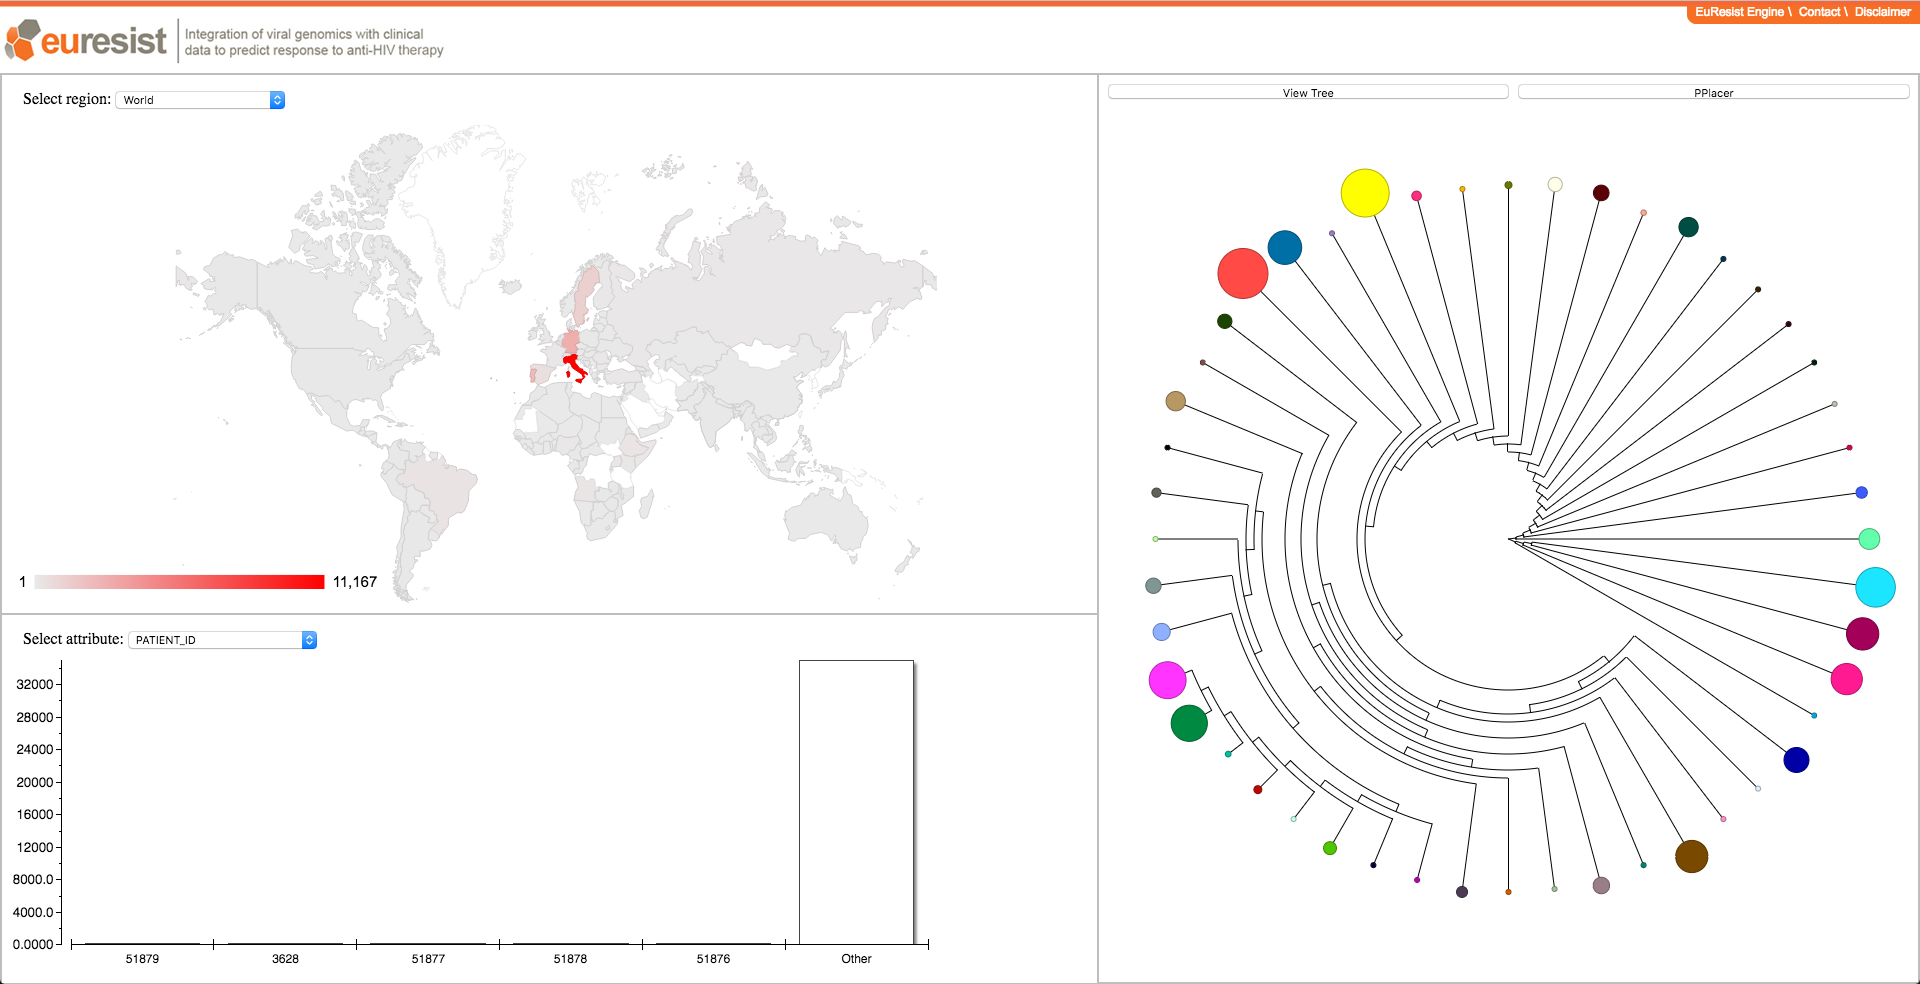
\includegraphics[scale=0.19]{images/defaultScreenshot.png}
\caption{Screenshot of the PhyloGeoTool application when the application is started for the first time.}
\label{fig:01} 
\end{figure}

%TODO (PL): Say something how this can actually be served (apache + tomcat, why: no tomcat on port 80.)

\section{Building from source}

\subsection{Prerequisites}
Install the Java Development Kit (JDK) with a version $\geq v 1.7$.\\

\noindent For example, on Ubuntu Linux, Oracle Java 8 can be installed as follows:
\begin{verbatim} 
sudo add-apt-repository ppa:webupd8team/java
sudo apt-get update
sudo apt-get install oracle-java8-installer
\end{verbatim}

\subsubsection*{Git}
Install git.\\

\noindent For example, on Ubuntu Linux, git can be installed as follows:
\begin{verbatim}
sudo apt-get install git-all
\end{verbatim}

\subsubsection*{Ant}
Install Ant version $\geq 1.9.4$ as we will use it to build the source code.\\

\noindent For example, on Ubuntu Linux, Ant can be installed as follows:
\begin{verbatim}
sudo apt-get install ant
\end{verbatim}

\subsection{Clone the git repository and build the JAR files and WAR file}
We here outline the various steps necessary for a successful build of the project.
\begin{itemize}
\item {Clone the git repository: 
\begin{verbatim}
git clone https://github.com/rega-cev/phylogeotool/
cd phylogeotool
\end{verbatim}
\item{Start the build process by running ant}
\begin{verbatim}
ant
\end{verbatim}
\item This build process generates a phylogeotool.war, DistanceMatrix.jar and PreRender.jar in the dist directory.
}
\end{itemize}

% TODO (GB) once published: write something like 
% Please cite ....

\section{Contact Information and support }


The PhyloGeoTool is developed and maintained by the Rega Institute KU Leuven.
You can contact us on \href{mailto:phylogeotool@kuleuven.be}{phylogeotool@kuleuven.be}

\end{document}
